\documentclass[aps,twocolumn,showpacs,preprintnumbers,nofootinbib,prl,superscriptaddress,groupedaddress]{revtex4-2}

% packages
\usepackage{amssymb,graphicx}
\usepackage{amsmath}
\usepackage{multirow}
\usepackage{epsfig}
\usepackage[usenames]{color} 
\usepackage[export]{adjustbox}
\usepackage{mathtools}
\usepackage{hyperref}
\usepackage{float}
\usepackage{placeins}



% you can define your own shortcuts etc, if you use sth very often
\newcommand{\balign}{\begin{align}}
\newcommand{\ealign}{\end{align}}

% or you can define your own symbols, check what this is
\def\meff{m_{\textrm{eff}}}


% here is where the document begins
\begin{document}

\title{PHYS 414 Final Project}
\author{G\"{o}rkem \c{C}avu\c{s}o\u{g}lu} % turkish characters require special handling
\affiliation{Department of Physics, Ko\c{c} University, \\
Rumelifeneri Yolu, 34450 Sariyer, Istanbul, Turkey }
\date{\today}

\begin{abstract}
\end{abstract}
\maketitle


%%%%%%%%%%%%%%%%%%%%%%%%%%%%%%%%%%%%%%%%
\section{Newton}
%%%%%%%%%%%%%%%%%%%%%%%%%%%%%%%%%%%%%%%%
%%%%%%%%%%%%%%%%%%%%%%%%%%%%%%%%%%%%%%%%


\subsection{(a) Analytical Derivations of Lane-Emden Equation}
Using Newtonian mechanics, two hydrostatic equilibrium equations are provided as
\begin{equation}\label{eq1}
	\frac{d m(r)}{dr}= 4\pi r^2 \rho(r)
\end{equation}
\begin{equation}\label{eq2}
	\frac{dp(r)}{dr} = -\frac{Gm(r)\rho(r)}{r^2}
\end{equation}
After rearranging terms of equation \ref{eq2} such that only $m(r)$ appears at right-hand side as a function of $r$, we obtain
\begin{equation}
	\frac{r^2}{\rho(r)}\frac{dp(r)}{dr} = -Gm(r)
\end{equation}
Taking derivatives of both sides, and using equation \ref{eq1} yield
\begin{equation}
	\frac{d}{dr}(\frac{r^2}{\rho(r)}\frac{dp(r)}{dr}) = -G\frac{dm(r)}{dr}= -4\pi G r^2 \rho(r)
\end{equation}
Thus, the equation is free of $m(r)$. Dividing both sides by $r^2$,
\begin{equation}
	\frac{1}{r^2}\frac{d}{dr}(\frac{r^2}{\rho(r)}\frac{dp(r)}{dr}) = -4\pi G  \rho(r)
\end{equation}
Using polytropic EOS $p = K\rho^{1+\frac{1}{n}}$, along with factorization $\rho(r) = \rho_c\theta^n(r)$ such that $p(r) = 
K\rho_c^{1+\frac{1}{n}}\theta^{n+1}(r)$,

\begin{align}
	\frac{K\rho_c^{\frac{1}{n}}}{r^2}\frac{d}{dr}(\frac{r^2}{\theta^n(r)}\frac{d}{dr}\theta^{n+1}(r)) = -4\pi G  \rho_c\theta^n(r) \\
	\frac{(n+1)K\rho_c^{\frac{1}{n}-1}}{4\pi G  }\frac{1}{r^2}\frac{d}{dr}(r^2\frac{d\theta(r)}{dr}) = -\theta^n(r)
\end{align}
If we use scaled radius such that $r = \alpha \xi$  where $\alpha^2 = \frac{(n+1)K\rho_c^{\frac{1}{n}-1}}{4\pi G  }$, we obtain the final form
\begin{equation}
	\frac{1}{\xi^2}\frac{d}{d\xi}(\xi^2\frac{d\theta(\xi)}{d\xi}) + \theta^n(\xi) = 0
\end{equation}

Using \texttt{Mathematica}'s asymptotic solve function \texttt{AsymptoticDSolveValue} to obtain a series solution of Lane-Emden equation, we obtain
\begin{equation}
\theta(\xi) \approx 1 - \frac{\xi^2}{6}+\frac{n\xi^4}{120}-\frac{(8n^2-5n)\xi^6}{1520}+\dots
\end{equation}

After this step, we can find closed-form analytical solutions of Lane-Emden equation. Evaluating Lane-Emden equation with \texttt{Mathematica}'s \texttt{DSolve} function for $n=1$ yields

\begin{equation}
	\theta(\xi) = \frac{sin(\xi)}{\xi}
\end{equation}


Since $M = \int_0^R 4\pi r^2\rho(r)dr = \frac{4\pi \rho_c}{\alpha^3}\int_0^{\xi_n} \xi^2\theta^n(\xi)d\xi$, substituting $\theta^n$ from Lane-Emden equation yields,
\begin{equation}
	M = 4\pi \rho_c\alpha^3\int_0^{\xi_n} -\frac{d}{d\xi}(\xi^2\frac{d\theta(\xi)}{d\xi})d\xi
\end{equation}
Evaluating the integral, and substituting $R = \alpha\xi_n$,
\begin{align}
&	M = 4\pi \rho_c\alpha^3[-\xi^2\frac{d\theta(\xi)}{d\xi}]\bigg|_0^{\xi_n} = 4\pi \rho_c\alpha^3\xi^3_n[-\frac{\theta'(\xi_n)}{\xi_n}] & \\
	&= 4\pi \rho_cR^3[-\frac{\theta'(\xi_n)}{\xi_n}] \label{eq13} & 
	% \nonumber forces that line to have no reference number
	% the ampersand (&) is used to align the lines. the places you put them are at the same position in each line.
\end{align}
For the stars sharing same polytropic EOS, $\frac{R}{\alpha\xi_n}=1$, then
\begin{equation}
	\frac{4\pi G}{(n+1)K \xi_n^2}\rho_c^{\frac{n-1}{n}}R^2 =1
\end{equation}
Since $K$, $n$, $\xi_n$ and others are constant for same polytropic equation except $\rho_c$, $\rho_c \propto R^{\frac{-2n}{n-1}}$ . \\
\begin{equation}
	M \propto \rho_cR^3 \to M \propto R^{3-\frac{2n}{n-1}}=R^{\frac{3-n}{1-n}}
\end{equation}

\newpage
\subsection{(b) Mass versus Radius Distributions of White Dwarfs}

Using \texttt{Python} for reading and plotting the given white dwarf, we obtain mass distributions as a function of radii. After calculating corresponding radii \texttt{R} for data, the distribution is plotted. 

\begin{figure}[!htb]
	\centering
	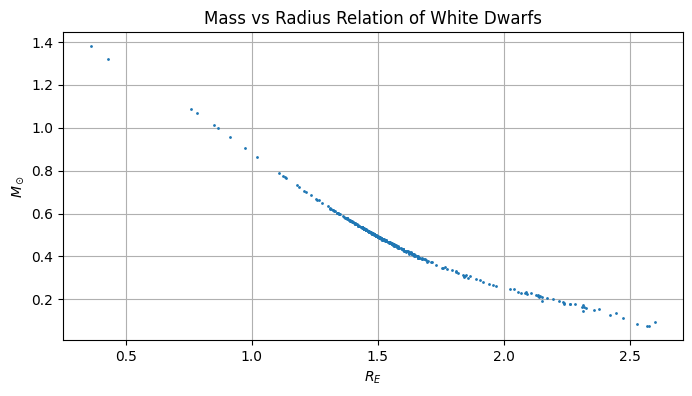
\includegraphics[width=1\linewidth]{Plots/newton-part-b}
	%\caption{}
	\label{fig:newton-part-b}
\end{figure}
\FloatBarrier

\subsection{(c) Obtaining Fitting Parameters for White Dwarf Data}

Given pressure equation for the white dwarfs,

\begin{equation}
	C(x( 2x^2 - 3)(x^2 + 1)^{-1/2} + 3sinh^{-1}(x))
\end{equation}

where $x$ is the scaled density parameter $(\frac{\rho}{D})^{\frac{1}{q}}$. After obtaining series expansion for the pressure as $x\to 0$ using \texttt{Mathematica}'s \texttt{Series} function, we get the leading parameter to approximate pressure for small $x$

\begin{equation}
	P \approx \frac{8C}{5}(\frac{\rho}{D})^{\frac{5}{q}}
\end{equation}

After arranging the leading term in the form $P \approx K_* \rho^{1+\frac{1}{n_*}}$, we obtain parameters $K_*$ and $n_*$ as,

\begin{align}
	n_* = \frac{q}{5-q} & \quad\quad\quad \And & K_* \frac{8C}{5D^{\frac{5}{q}}}
\end{align}

After fitting the white dwarf data in \texttt{Python} for integer $q$, we obtain $q=3$ and using fitting parameters, we can plot the curve for small $M$

\begin{figure}[!htb]
	\centering
	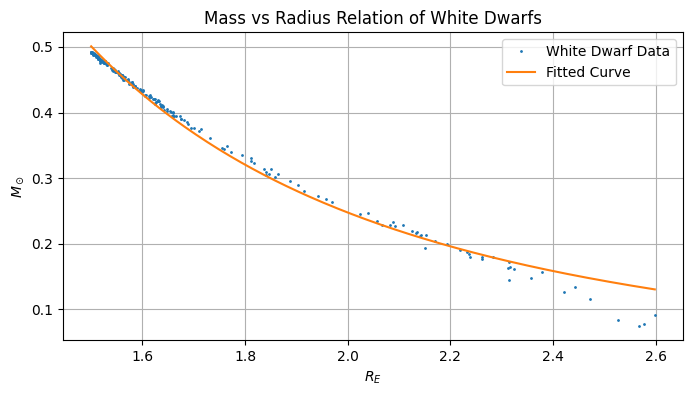
\includegraphics[width=1\linewidth]{Plots/newton-part-c1}
	%\caption{}
	\label{fig:newton-part-c1}
\end{figure}
\FloatBarrier

Numerically solving Lane-Emden equation in \texttt{Python}, we obtain the solution for $n=\frac{3}{2}$ given below 

\begin{figure}[!htb]
	\centering
	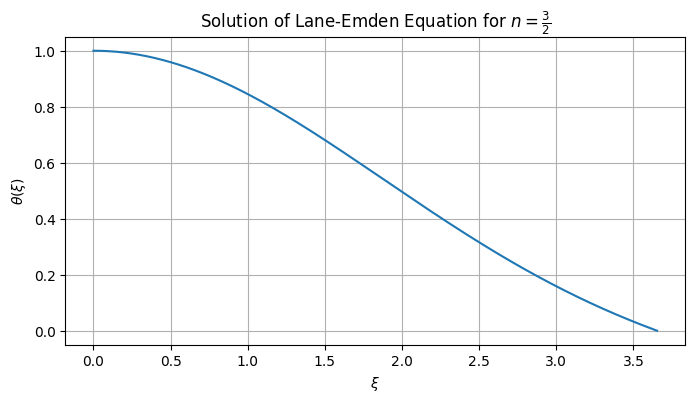
\includegraphics[width=1\linewidth]{Plots/newton-part-c2}
	%\caption{}
	\label{fig:newton-part-c2}
\end{figure}
\FloatBarrier

By calculating the central densities of white dwarfs using \ref{eq13} and numerical solutions of Lane-Emden equation, we obtain the plot

\begin{figure}[!htb]
	\centering
	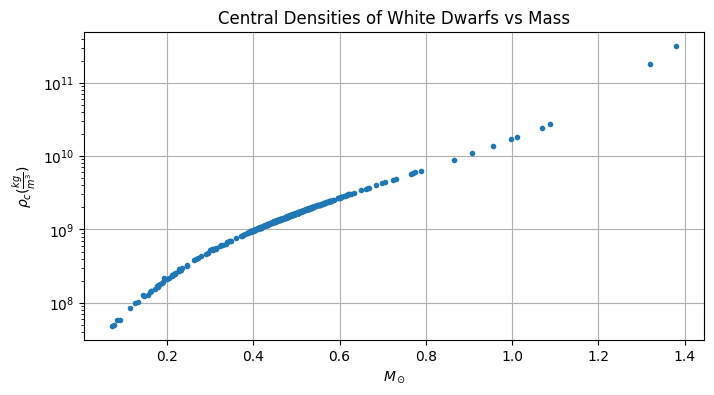
\includegraphics[width=1\linewidth]{Plots/newton-part-c3}
	%\caption{}
	\label{fig:newton-part-c3}
\end{figure}
\FloatBarrier

After fitting the data for parameter $K$, we obtain $K = 2774995.74$ and using the parameters, we plot the fitting curve

\begin{figure}[!htb]
	\centering
	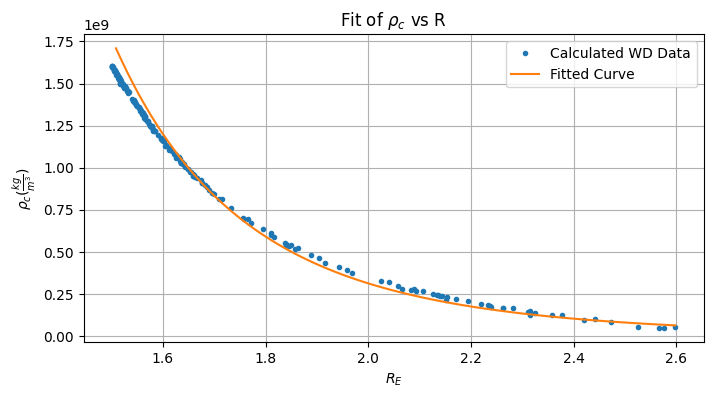
\includegraphics[width=1\linewidth]{Plots/newton-part-c4}
	%\caption{}
	\label{fig:newton-part-c4}
\end{figure}
\FloatBarrier

\subsection{(d) Obtaining the Parameters C and D by Interpolation}

Using interpolation and solving IVPs using hydrostatical differential equation $\frac{dm}{dr} = 4\pi r^2 \rho$ and the equation reduced for $\rho$

\begin{equation}
	\frac{d\rho}{dr} = -G \frac{\sqrt{x^2+1}}{8Cx^5}\frac{qm\rho^2}{r^2}
\end{equation}

we obtained that $D = 3022830886$ and C = $1.96 \cdot 10^{22}$. Theoretical values of them were $D = \frac{m_{u}m_{e}^{3}c^{3}\mu_{e}}{3\pi^{2}\hbar^{3}} \approx 3934510$ and $C = \frac{m_{e}^{4}c^{5}}{24\pi^{2}\hbar^{3}} \approx 2.43 \cdot 10^{19}$. Approximately a thousand times of theoretical constants are found in the numerical calculation.

\subsection{(e) Obtaining the Complete Numerical Solution for Mass and Radii}

Using obtained parameters $C$ and $D$, numerical solution of white dwarf mass-radius relation is plotted as

\begin{figure}[!htb]
	\centering
	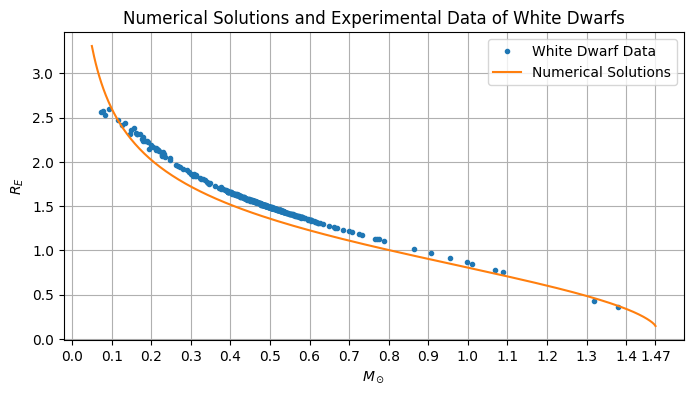
\includegraphics[width=1\linewidth]{Plots/newton-part-e}
	%\caption{}
	\label{fig:newton-part-e}
\end{figure}
\FloatBarrier

Chandrasekhar mass $M_{Ch}$ is found as $1.47M_\odot$.

\section{Einstein}

\subsection{(a) Numerical Solutions of Tolman–Oppenheimer–Volkoff Equations}

Using given polytropic definition of pressure $P = K\rho^2$, TOV equations converted into:

\begin{align}
		&\frac{dm}{dr} = 4\pi r^2\rho   & \\
	&\frac{d\nu}{dr} = 2\frac{m+4\pi K\rho^2r^3}{r(r-2m)}  &  \\
	&\frac{d\rho}{dr} = -\frac{m+4\pi K\rho^2 r^3}{r(r-2m)}\frac{1+K\rho}{2K} = -\frac{1}{2}\frac{1+K\rho}{2K}\nu'  &
\end{align}

Such that there is not explicit P-dependence. Instead of pressure, we can directly solve the TOV equations for density. Given initial conditions $\rho(0)=\rho_c$, $m(0)=0$, and $\nu(0)=0$, the coupled equations are integrated with \texttt{SciPy}'s \texttt{solve\_ivp} function. For provided central density values, mass and radii of neutron stars are obtained. The curve of mass-radius relation of neutron stars is given below.

\begin{figure}[!htb]
	\centering
	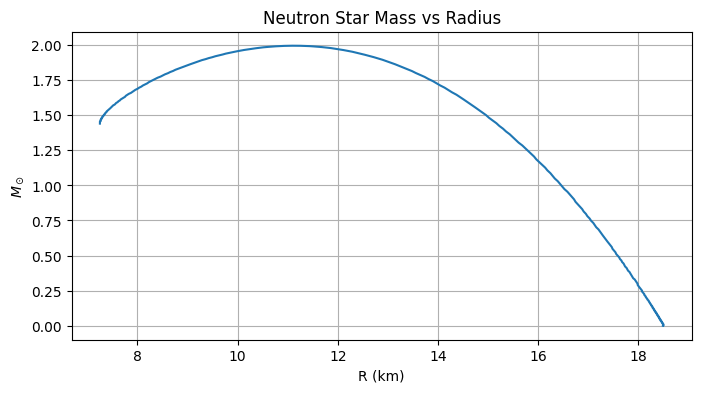
\includegraphics[width=1\linewidth]{Plots/einstein-part-a}
	%\caption{}
	\label{fig:einstein-part-a}
\end{figure}
\FloatBarrier
\subsection{(b) Baryonic Mass and Fractional Binding Energy}

Baryonic mass of the neutron stars are calculated by appending the equation \ref{eq23} to TOV equations,

\begin{equation}\label{eq23}
	\frac{dm_P}{dr} = 4\pi (1-\frac{2m}{r})^{-1/2}r^2\rho
\end{equation}

Fractional binding energy of the neutron stars is also given as $\Delta=\frac{M_P-M}{M}$. The plot of fractional binding energy for varying radii is provided below.

\begin{figure}[H]
	\centering
	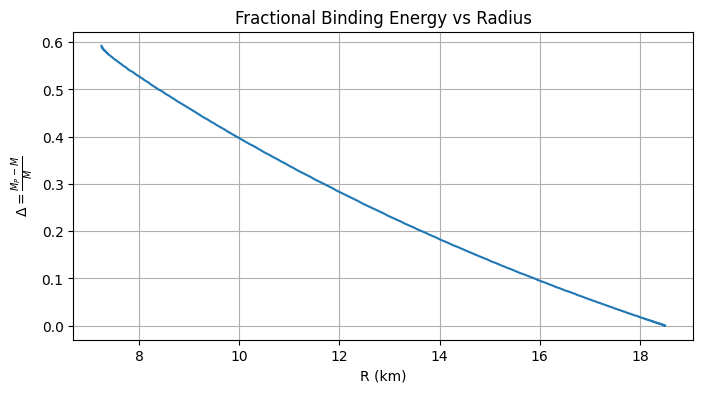
\includegraphics[width=1\linewidth]{Plots/einstein-part-b}
	%\caption{}
	\label{fig:einstein-part-b}
\end{figure}
\FloatBarrier

\subsection{(c) Stability of the Neutron Stars}

The stability condition is given as $\frac{dM}{d\rho_c} > 0$. On our specific case, that $\rho_c$ is always increasing, thus $d\rho_c$ is always greater than zero. Then, reduced stability condition is $dM > 0$. Although the derivative can be calculated as an irregular derivative, in our specific case, the condition is simplified. $\Delta M$ is calculated using numerical differencing. The obtained stability curve of the neutron stars is provided below.

\begin{figure}[H]
	\centering
	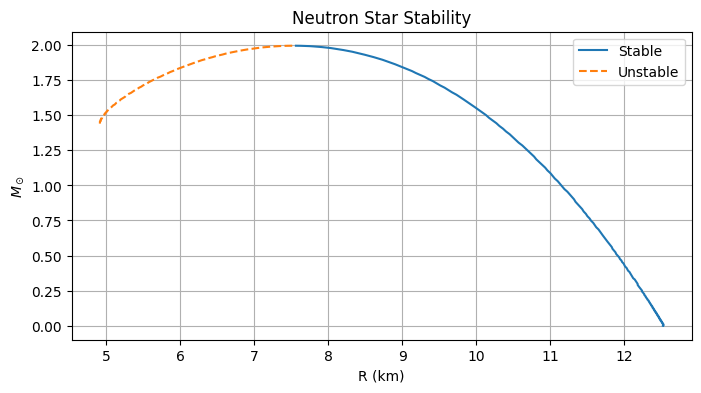
\includegraphics[width=1\linewidth]{Plots/einstein-part-c}
	%\caption{}
	\label{fig:einstein-part-c}
\end{figure}
\FloatBarrier
\subsection{(d) Maximum Neutron Star Masses}

Maximal mass of neutron stars described by polytropic equation depends on the value of constant $K$. For $K = 100$, $M_{max} \approx 2$. Although maximal masses increase with increasing K, maximum observed neutron star mass $2.14M_\odot$ limits K. Calculations yield that maximum of allowed value of K is 114. Above this value, neutron star masses exceed the maximum observed value. Maximal mass depending on varying K values are provided below.

\begin{figure}[H]
	\centering
	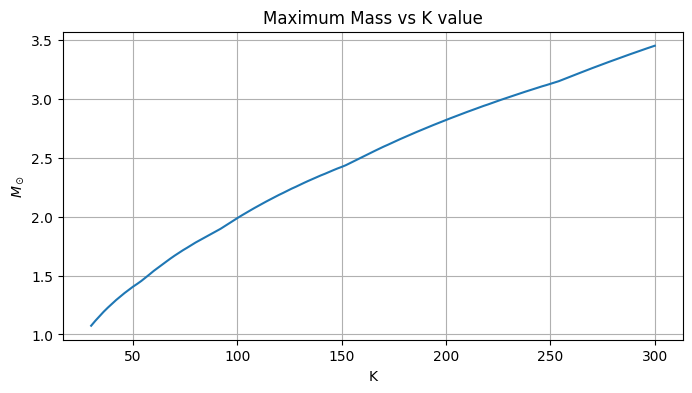
\includegraphics[width=1\linewidth]{Plots/einstein-part-d}
	%\caption{}
	%\label{fig:einstein-part-d}
\end{figure}
\FloatBarrier

\subsection{(e) TOV Equation outside of Star}

The differential equation of parameter $\nu$ outside of the star is reduced to the form
\begin{equation}
	\frac{d\nu}{dr} = \frac{2M}{r(r-2M)}
\end{equation}
Since we can factorize right-hand side as $\frac{1}{r-2M}-\frac{1}{r}$, we collect variables and differentials side by side, and put under integral sign as

\begin{equation}
	\int_R^{r}d\nu  =\int_R^{r}\frac{dr'}{r'-2M}-\int_R^{r}\frac{dr'}{r'}
\end{equation}

After integrating, we obtain

\begin{equation}
	\nu(r)-\nu(R)  = ln(r-2M)-ln(R-2M)-(ln(r)-ln(R))
\end{equation}
Then simplifying it yields the final form for $r > R$

\begin{equation}
	\nu(r > R)  = ln(1-\frac{2M}{r})-ln(1-\frac{2M}{R}) + \nu(R)
\end{equation}

\end{document}
